%% modified ieee for AI
%% K. Pucejdl 2017

\documentclass[journal]{IEEEtran}
\usepackage{graphicx}
\usepackage{epstopdf}
\usepackage{subcaption}
\usepackage[utf8]{inputenc}
\usepackage[czech, english]{babel}	
\usepackage{amsmath}
\usepackage{hyperref}

% Prettyref package
\usepackage{prettyref}
\newrefformat{ch}{Chapter~\ref{#1}}
\newrefformat{sec}{Section~\ref{#1}}
\newrefformat{ssec}{Subsection~\ref{#1}}
\newrefformat{fig}{Fig.~\ref{#1}}
\newrefformat{eq}{Eq.~(\ref{#1})}
\newrefformat{tab}{Tab.~\ref{#1}}
\newcommand{\refp}[1]{\prettyref{#1}}

% Macros and other useful commands
\newcommand{\e}[1]{\, e^{#1}}
\newcommand{\mat}[1]{\mathbf{#1}}
\newcommand{\vect}[1]{\mathbf{#1}}
\newcommand{\sub}[1]{_\mathrm{#1}}

\begin{document}
	
	\title{Benchmarking different hardware architectures using a parallel implementation of the N-Body Simulation algorithm}
	\author{{Jan \textsc{Mrázek}}, {mrazeja7@ksu.edu}}
	
	\markboth{Course project, CIS 750 - Advanced Computer Architecture Experiments, Kansas State University, Fall 2017}{Shell \MakeLowercase{\textit{et al.}}: Bare Demo of IEEEtran.cls for Journals}
	\maketitle
	
	\begin{abstract}
		
		This is a write-up paper which describes my efforts when working on a course project for the Advanced Computer Architecture Experiments course at Kansas State University during the Fall 2017 semester.
		
		First, the N-Body Simulation problem is described. As there are multiple ways of simulating a system of large amounts of space bodies, two different algorithms are presented and their pros, cons, accuracy, time complexity and implementation difficulty are compared. 
		
		One of the algorithms is then implemented in a simple, naive way and then optimized, parallelized and custom-tuned to run on computer chips of very different architectures. 
		
		This optimization is done in multiple iterations, each time with explanations regarding the relative speedups and overall performance.
		
		Finally, multiple different versions of the algorithm are run on computer hardware of different architectures, and the resulting data is analyzed and commented on. Performance is measured in the amount of billions of floating-point operations (gigaFLOPs) per second, and the efficiency of each computer chip is addressed. An overall conclusion is drawn which compares the results gathered during the benchmarking phase of the project.
		
	\end{abstract}

	\section{Project Proposal}
		
		In my course project, I explored the ins and outs of efficient parallel design and better cache-friendliness when it comes to programming techniques when applied on different CPU architectures. After briefly describing the N-Body simulation and two different algorithms which can be used to solve it, I chose one and implemented it in the C++ language. I then fine-tuned the source code to better suit each CPU architecture that was tested. Then I benchmarked all of the different implementations that I created and commented on the (sometimes vast) performance differences and speedup yields between them.	
	
	\section{Problem definition}
	
		\subsection*{The N-Body simulation}
		
			The N-body simulation is a way to simulate continuous gravitational interactions among potentially very large amounts of galactic bodies, solar systems and similar particles, where every single body influences the positions and velocity vectors of all other bodies. It is a tool that is used widely and frequently in the fields of astronomy and astrophysics to help researches reach a better understanding of the evolution of a large-scale structure of the universe.\cite{scholarpedia}		
	
	\section{Problem background and scope}
	\label{algs}
	
		\subsection*{Choosing an algorithm}
	
			There are many ways to go about the problem of implementing a suitable algorithm for the simulation of space particle movements. 
			
			The first thing that we have to think about when it comes to making a choice in this matter is the trade-off between a relatively reasonable time-complexity of the algorithm and the scientific accuracy of the algorithm according to the laws of physics that is required.
			
			If we needed to run a truly massive (hundreds of millions to billions of space bodies) N-Body movement simulation for a high amount of iterations, it would be best to choose the Barnes-Hut algorithm. If instead we prioritize complete accuracy of all computations above all and don't really mind extremely long running times on the same amount of bodies for the same amount of iterations, it is best to stick with an algorithm that solves the simulation in a brute-force, but accurate manner.
	
		\begin{figure}[ht]
			\centering
			\includegraphics[width=0.5\textwidth]{sandbox2.jpg}
			\caption{An illustration of an orbital timelapse in \textit{Universe Sandbox$^2$}}
			\cite{nbodypic}
		\end{figure} 
	
		\subsection*{Brute-Force algorithm}
			The most obvious and most accurate algorithm of solving the N-body simulation is simply a brute-force approach. This algorithm makes sure to compute the forces that are being applied between all pairs of space particles within a given system, thus ensuring scientifically correct movements. This algorithm is also sometimes called "the all-pairs N-Body simulation algorithm."
			
			In the computation of each iteration, or time step, we calculate force vectors $\textbf{f}_{ij}$. $\textbf{f}_{ij}$ signifies the force that is applied on body $i$ caused by its gravitational pull on a different body $j$. 
			
			Given $\textbf{n}$ bodies with an initial position vector $\textbf{p}_{i}$ for 1$ \leq i \leq \textbf{n}$, the force vector $\textbf{f}_{ij}$ is given by the following formula \cite{nvidia-article}:
			
			\begin{equation}
			\centering
				\textbf{f}_{ij} = K \frac{m_i m_j \cdot r_{ij}}{||r_{ij}||^2} 
			\end{equation}
			
			where $m_i$ and $m_j$ are the respective masses of bodies $i$ and $j$; $r_{ij}$ is the length vector between bodies $i$ and $j$, i.e. $r_{ij} = p_j - p_i$, and $K$ is the gravitational constant used in the simulation; $K = 6.674 \cdot 10^{-11}$ \cite{constant}. As you can see from the equation above, the force vector is not linear; instead, the relative force pulling on body $i$ diminishes with the square of distance between these two bodies (or the vector $r_{ij}$).
			
			The total force that acts on body $i$ - $\textbf{F}_i$ - while it interacts with all other $\textbf{n}-1$ bodies, is given by the sum of all particular force vectors:
			
			\begin{equation}
			\centering
				\textbf{F}_i = \sum_{j = 1}^{N}\textbf{f}_{ij}
				 = K m_i \sum_{j = 1}^{N}{\frac{m_j \cdot r_{ij}}{||r_{ij}||^2}}
			\end{equation}
			
			\subsection*{Time complexity}
			
				Of course, being a brute-force algorithm, the asymptotic bound on computation time is not very good. Because the algorithm needs to touch all particle pairs during a single iteration of the computation, the time complexity is bounded by $O(k \cdot n^2)$, where $k$ is the number of iterations, or time steps we simulate for, and $n$ stands for the number of bodies there are in the given system.
		
		\subsection*{Barnes-Hut algorithm}
		\label{barnes}
			
			The Barnes-Hut algorithm offers a very different approach to solving the simulation in a timely, yet less accurate manner. This algorithm is a mere approximation of the N-Body simulation problem, which implies that it is best used when the running time of the computation is a significant constraint and the physical accuracy of the simulation is maybe not as important.
		
			The Barnes-Hut algorithm divides the whole space of the given system into different quadrant cells. The algorithm then only calculates the forces between particles within a single cell, not taking into consideration any other single particles. For quadrant cells where the number of bodies occupying it is particularly small, the brute-force algorithm is used to solve the simulation instead, as it is inefficient to divide the space within the quadrant cell any more.
	
			\begin{figure}[ht]
				\centering
				\includegraphics[width=0.5\textwidth]{barneshut.png}
				\caption{\label{cells}An illustration of the Barnes-Hut quadrant division}
				\cite{barnespic}
			\end{figure}
	
			All other cells are then each treated as one massive body, which has the mass of all particles contained within a given cell. The position of this dense uber-body is centered around the center of mass of all neighboring particles within that cell. Other than this important modification, the algorithm still works very similarly to the brute-force algorithm. 
			
			The fact that only a single massive body is sometimes used instead of many other smaller bodies in the computation drastically reduces the number of pairs whose influences have to be calculated. The time complexity of the Barnes-Hut algorithm is thus bounded by $O(k \cdot n \cdot log n)$, where $k$ is the number of time steps we simulate for, and $n$ is the number of bodies there are in the given system.
			
			It is important to also mention the drawbacks of this algorithm. Because of the approximated mass of a majority of the particles during a single iteration, the Barnes-Hut algorithm is not very accurate in the scientific sense. 
			
			Apparently, the recursive nature of the algorithm also makes it somewhat unsuitable for parallel implementations, meaning that the brute-force algorithm might actually perform better on a massively multi-threaded machine for systems with reasonably low numbers of space bodies.
			
		These reasons are why I chose to pursue the implementation, optimization and parallelization of the brute-force algorithm over the Barnes-Hut algorithm.
	
	\section{Related work in literature}
	
		Typical N-Body simulation problems can be traced all the way back to the 1960s. The first astrophysical simulation of this kind was performed by Sebastian von Hoerner in 1960 for a dynamic system consisting of just 16 particles. \cite{camb_book}
		
		At that time, the lack of computational facilities meant that scientists had to decide between performing fewer interations of the simulation with the highest amount of particles ($n$)  possible, or perform a much more in-depth study of significantly smaller systems.\cite{camb_book}
		
		A milestone of an even amount of $n=100$ bodies was reached by S. J. Aarseth in 1962. Another milestone of $n=500$ for spherical liquid bodies was reached in 1964 by A. Rahman. \cite{history}
		
		Since those times, it can be said that the performance of N-Body simulations has been limited by Moore’s law and therefore advancements in moden computer architectures. A significant single-machine speedup was reached with the introduction of multi-core processors. Another fairly large (and fairly recent) leap in computational performance was caused by the dawn and spread of graphics processing units (GPUs) and their use for scientific calculations. Technologies like OpenCL and CUDA have been extremely helpful in all kinds of topics in the field of scientific computation.
		
		N-Body simulations have been at the forefront of high-performance computing in the terms of \textit{FLOPs/s} (or floating point operations per second) that they deliver.\cite{history} This is especially true for the brute-force (or all-pairs) N-Bbody algorithm, as it responds fairly positively to parallelization efforts. 
		
		There have been discussions whether the FLOPs/s metric is even useful in the comparison of these algorithms, or whether the "amount of science done" should somehow be considered instead. Other algorithms, such as the Barnes-Hut algorithm, may be less efficient theoretically, but they can deliver more "information" in the same amount of computation time.
		
		Nowadays, it is possible to simulate dynamic systems with as many as $10^{11}$ space particles. In 2010, a team of programmers at Nagasaki University in Japan created a parallel implementation of the N-body problem using NVIDIA’s CUDA technology. When the massively parallel implementation was ran on a supercomputer containing a total of 576 \textit{GT200} (Tesla 2.0 architecture) GPUs, they measured a performance of 190.5 \textit{TFLOP/s}. \cite{teraflops}
		
		The theoretical processing power of such a supercomputer should be in the neighborhood of about 580 TFLOPs/s, as one GT200 chip can perform as many as (depending on core configuration and clock speeds) 1010 GFLOPs/s.\cite{wikitesla}
		
		The resulting 190.5 TFLOPs/s is a very respectable number, especially since the code that was used to run the computation used the Barnes-Hut algorithm, instead of the "faster" (FLOPs/s- or performance-wise) brute-force method.
		
	\section{Methods and facilities used}
	
		Before I started working on this semestral project, I planned to first implement a naive version of the brute-force N-Body simulation algorithm. Then I wanted to work iteratively in an effort to optimize the source code in order to take better advantage of a computer's memory hierarchy, more specifically the CPU's caches. 
		
		I decided to use the C++ programming language to write all of my source code where applicable, and for the CUDA part of my implementation, I would use NVIDIA's CUDA-C language, which is actually just C/C++ with a little bit of extra functionality. I also took advantage of C++'s C++11 standard, which brings a lot of new features into the language compared to its previous versions. In order to get very accurate timing results during my benchmarking efforts, I used C++11's \texttt{<chrono>} library. I could have used other, older libraries to do this task, but I wanted to try a new approach, even when it comes to an area that probably doesn't offer much improvement anymore.
		
		Then I wanted to transform the code using the OpenMP parallel programming interface, and finally, if time permitted, create an implementation that would use NVIDIA's CUDA technology.
		
		I planned on testing and benchmarking the computing performance of all of these proposed versions on the following hardware:
		
		\begin{itemize}  
			\item[-]{a typical personal computer CPU architecture, i.e. Intel’s x86-64. I planned to use Kansas State University’s Beocat supercomputer to run the tests on this architecture.}
			
			\item[-]{an ARM-architecture based computer. I wanted to use my own OrangePi One micro-computer, which had been  setup as a media center in my home. This micro-computer uses a single Allwinner H3 SoC (system-on-chip) with a quad-core processor and an integrated GPU. The CPU's clock speed is 1200 MHz. I planned to install a fresh distribution of the ARMbian OS on it and run all of my tests that way.}
			
			\item[-]{a computer equipped with Intel’s Xeon Phi coprocessor card. I hoped to confirm my theoretical knowledge I have about this coprocessor card – that it is extremely suitable for simple, embarrassingly parallel computations and vector computing. I hoped to see a significant speedup compared to Intel’s x86-64 architecture. I planned to run my tests on a Xeon Phi-equipped computer at my home university (Czech Ttechnical University in Prague, Czech Republic).}
			
			\item[-]{I also wanted to run a CUDA implementation on a computer equipped with an NVIDIA graphics processor. I hoped to run these benchmarks on nodes that are part of Beocat and have dedicated GPUs just for this purpose. I ended up having to settle to running my benchmarks on a significantly slower consumer-grade GPU in the end.}
		\end{itemize}
	
	\section{Breakdown of tasks, time and work schedule}
	
		The first step I needed to take was the implementation of a really simple, unoptimized, sequential N-body simulation algorithm. 
		
		The next task on my plan was the integration of some sort of graphical interface that I would use to better understand the exact happenings during my calculations, and to possibly help debug the algorithm's implementation. Another good side that I thought it would bring to the project is the fact that it would look
		
		After obtaining a working naive sequential implementation of the project, I planned to start my work on redesigning the algorithm in a more efficient manner. I wanted to try to apply my knowledge that I gained duriny the semester in CIS 750 in order to maximize the usage of all system resources, which of course includes the usage of a parallel interface, which was also a step that I needed to take. I planned to integrate the OpenMP parallel programming interface into the code, as well as directives used to run programs on the Xeon Phi coprocessor card (with use of Intel's C++ compiler).
		
		Of course, I also planned to create a parallel version of my implementation using NVIDIA’s CUDA technology.
		
		I would then test and measure running times with a variable amount of cores used for the computation and a variable number of bodies. I wanted to ideally try to collect a large amount of data to get a better grasp on the overall performance of the algorithm when used on different machines and chips.
		
		The last step in my course project would be the analysis of data that was to be gathered.
		
		To put my proposed work schedule into perspective, you can take a look at the Gantt chart in figure \ref{gantt}.
		
		\begin{figure}[ht]
			\centering
			\includegraphics[width=.5\textwidth]{gantt.png}
			\caption{\label{gantt}Gantt chart of the proposed estimated project work schedule}
		\end{figure} 
		
	\section{Project progress: Naive implementation}
	
		The first task on my plan was the implementation of a naive version of the brute-force N-Body simulation algorithm. 
		
		I chose to write the naive version in such a way that it would be very easily readable and simple to understand. I created a \texttt{Body} class that represents each individual body object and all of its properties (those being the postion vector, velocity vector and mass). This class also contains an \texttt{updatePhysics()} method, which essentially calculates the $\textbf{f}_{ij}$ force vector for any body $j$ that is passed to the method as an argument. The whole system used in the simulation is contained in the \texttt{Simulation} class. This class contains a \texttt{vector} of all bodies in a given system, as well as additional properties used for the simulation, such as the number of iterations that have passed since the beginning, or a method that takes care of randomly generating a given number of bodies.
		
		I quickly benchmarked this early version of the implementation and found out that it produces a computing performance of about $5$ GFLOPs/s when run on a single core on K-State's Beocat supercomputer.
		
		\subsection*{GIF animations}
		
			A utility that I also used a lot of the time when creating and debugging the naive implementation was the GIF-making library for C/C++ created by Charlie Tangora. \cite{gif}
			
			Using this library, I could see the results of any edits I made in the source code almost immediately. I integrated the library in such a way that it is very simple to generate an animated image in \texttt{.gif} format with given dimensions and number of frames. The background of this animated image is always black, with all bodies being represented as green dots. The shade of green of these dots is also scaled to reflect the mass of each body in the system.
		
	\section{Project progress: Structure of arrays}
		
		After having completed the naive implementation, I took a look at redesigning pretty much the whole source code in order to take advantage of the CPU's cache.
		
		I thought about the concept of spatial locality of data in the cache, and decided to ditch the object-oriented design of my simulation. I ended up changing my whole approach to storing data in memory. Instead of keeping on using an "array of structures" kind of design that is easy to understand at a glance, I rewrote the code to represent a "structure of arrays" approach. In reality, I got rid of nearly the entire class structure of the code, and instead used dynamically allocated arrays to store the attributes of all bodies. I implemented different arrays that each stored one of the parameters for all bodies within the system. This way, the spatial locality concept of the cache can be taken advantage of during the force vector calculations.
		
		\subsection*{Resulting speedup}
			After running some very quick benchmarks and comparing the results to the previous unoptimized version, I found out that this improved version of my simulation boasts an approximately 10\% higher performance when compared to the previous object-oriented approach depending on the simulation size (i.e. body count and number of iterations).
			
			You can see the differences in the performance of these two designs in figure \ref{oopsoa}.		
			
			\begin{figure}[ht]			
				\centering
				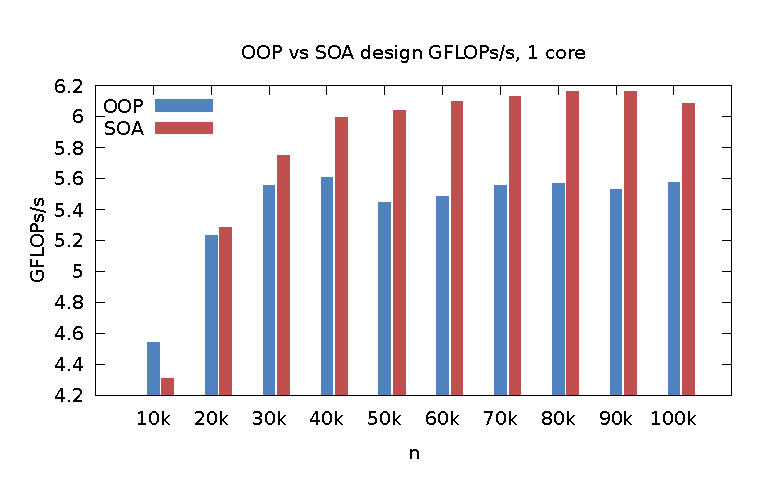
\includegraphics[width=.5\textwidth]{gnuplot/oop_vs_arr.eps}
				\caption{\label{oopsoa}Performance comparison of OOP and SOA approaches}
			\end{figure} 
	
	\section{Project progress: Parallelization with OpenMP}
	
		After redesigning the application to make better use of the CPU's cache, I took a look at parallelizing the code.
		
		As the machines I would use to benchmark the program contain multiple processors each with a significant amount of computing cores, not taking advantage of them would mean a loss of a huge amount of performance.
		
		With help from the OpenMP parallel programming interface, I changed the code in a way that the force vector calculations could be performed almost completely independently in different CPU threads. To make this possible, I used the \texttt{\#pragma omp parallel for} directive, which automatically parallelizes a \texttt{for} loop. Using the \texttt{schedule(dynamic)} clause, I told the compiler to schedule each iteration of the \texttt{for} loop dynamically. From running some quick tests, I found that this approach was slightly more efficient (a performance gain of about 3\%) than static or any other form of scheduling. I also used the \texttt{\#pragma omp simd reduction} clause to take advantage of some of the vector instructions that all modern x86 CPUs have. Using this directive also further helps the compiler vectorize \texttt{for} loops.
		
		\subsection*{Resulting speedup}
			To benchmark and verify the speedup and effectiveness of my efforts to try to parallelize the application using OpenMP, I ran a multitude of benchmarks, all on Beocat.
			
			I mainly ran benchmarks that measured the simulation's speedup depending on the number of threads being used. I also ran all of these tests with variable numbers of bodies in the simulation. You can see a graph of some of my results in figure \ref{parspeedup}. 
			
			\begin{figure}[ht]			
				\centering
				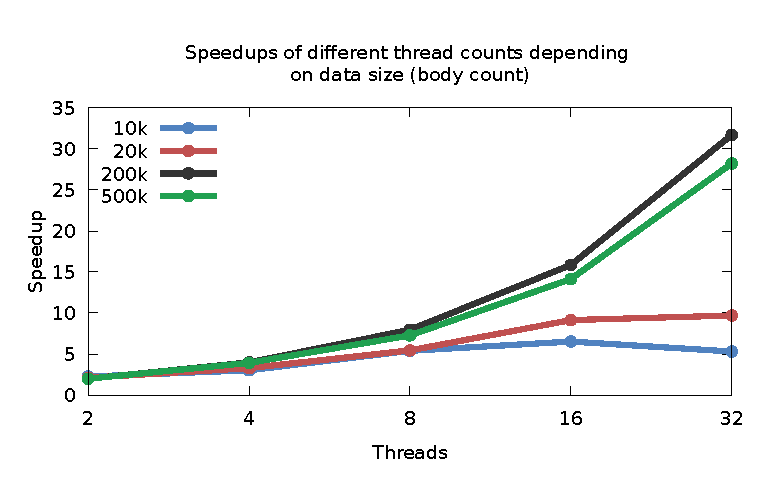
\includegraphics[width=.5\textwidth]{gnuplot/speedup.eps}
				\caption{\label{parspeedup}Parallel speedups when using OpenMP depending on number of threads and bodies}
			\end{figure} 
			
			I decided to only pick a couple of data points - you can see the speedups when using $2-32$ threads when compared to just a sequentially run application with either $10$, $20$, $100$ or $500$ thousand bodies, respectively. It is apparent that for large amounts of bodies, the speedups get even higher, reaching almost linear levels. The best speedup I measured when using 32 threads was $31.69$, which is extremely good and can't really be improved much further.
			
			The sometimes amazing speedups I measured are definitely due to the embarrassingly parallel nature of the brute-force N-Body simulation algorithm, but also due to the high efficiency of all compiler optimizations, vectorization and the OpenMP interface.
			
	\section{Project progress: Intel Xeon Phi}
	\label{phisection}
		
		After I was dont with the implementation and benchmarking of the OpenMP parallel version of the N-Body simulation project, it was time to start rewriting the program once again for use on the Intel Xeon Phi coprocessor card.
		
		The exact piece of hardware I used was a Xeon Phi 7120X. It is based on the Knight's Corner architecture, which was unveiled in 2013. It is indeed not the freshest piece of hardware, but it will do just fine.
		According to Intel's specifications page, ARK\cite{ark}, this specific coprocessor card contains 61 independent CPU cores, each clocked at $1.24$ to $1.33$ GHz. It also features a different type of Hyper-Threading technology than Intel's typical CPUs, as each core takes care of up to 4 threads at once. This means that your program can effectively take up 224 threads in all. It also has 16 gigabytes of GDDR5 memory and a 512-bit memory bus. The theoretical maximum floating-point performance of this particular Phi is $650.5$ GFLOPs/s \cite{tpu}.
		
		I ran all benchmarks that were using this device on a small computing cluster back at my home university, the Faculty of Electrical Engineering of the Czech Technical University.
		
		\subsection*{Implementation specifics}
		
			Since the source code that I'd developed until this point was already pretty solid when it came to efficient memory usage, I didn't have to change the code too heavily in order to use the Xeon Phi coprocessor efficiently. As the Xeon Phi largely uses OpenMP, I was able to left the parallelised code I had written earlier in with no modifications. I mainly added some additional directives that helped the device and Intel's compiler link the code. I opted to align all data arrays in order to help take advantage of vectorization; I used the \texttt{\_\_attribute\_\_((aligned(256)))} clause when defining each property array to let the compiler know that the corresponding data is properly aligned and can be safely vectorized.
			
		\subsection*{Resulting data and speedups}
		
			Benchmarking the Xeon Phi-friendly code was pretty straightforward. I mostly recycled all of the benchmarking scripts that I used in my previous tests. 
			
			I used dataset sizes that were identical to all of my previous benchmarks, and after I measured all running times and calculated the resulting performance in GFLOPs/s, I made the chart you can see in figure \ref{32_vs_phi}. In it, I made a simple bar graph that illustrates the difference in performance between the Xeon Phi version of my simulation and the previous OpenMP implementation running on 32 threads on a typical x86-64 architecture.
			
			\begin{figure}[ht]			
				\centering
				\includegraphics[width=.5\textwidth]{gnuplot/phi_vs_32.eps}
				\caption{\label{32_vs_phi}Comparison of 32-thread CPU and Xeon Phi}
			\end{figure} 
			
			Even though the Xeon Phi uses nearly 8 times the number of threads, it only managed to be approximately $2.3$ times as fast as the regular CPU. This is definitely caused by the whole nature of this architecture; instead of depending on a relatively small number of very complex CPU cores, the Xeon Phi relies on a bigger number of very simple cores which operate on a shared memory. It also runs at a much slower clock rate, about a third to a half of that of the regular Xeon CPUs that I used for my previous tests. Its microarchitecture is also quite a bit older than the CPUs I used, which also causes a non-insignificant performance difference.			
			
			When taking into consideration the device's maximum floating-point performance of $650.5$ GFLOPs/s, my maximum achieved performance of $393$ GFLOPs/s is really good. It only reaffirmed the fact that the brute-force N-Body simulation algorithm is computationally not very complex and quite embarrassingly parallel.
			
			Even though the overall running times compared to a "regular" CPU architecture weren't as impressive as I had hoped, I am still glad I could measure the differences between these two wildly different architectures.
		
	\section{Issue: ARM-based device}
	\label{orangepi}
	
		The next part of my project was the addition of results to be gathered from running benchmarks on a device equipped with an ARM-architecture based CPU. For this part of the project, I had picked an OrangePi One development board. This board has a quad-core Allwinner H3 SoC clocked at approximately $1.2$ GHz, 512 megabytes of memory and a TDP of approximately 10 watts. I was looking forward to seeing just how much slower this architecture is to any other kind of contemporary architecture.
		
		I ran into quite a big issue, though; the OrangePi device I owned and planned to use ended up not being reachable via \texttt{ssh}. After investigating further, it turns the power supply part of its circuitry had failed and thus it wouldn't run at all. I ended up not bothering with trying to revive the device and just skipped this part of the project altogether. Take these two paragraphs as a sort of an excuse for any results that are missing.
	
	\section{Project progress: CUDA implementation}
	\label{cudasection}
	
		After I was done with all other benchmarks (excluding the ARM architecture for reasons mentioned earlier), I proceeded to create one last implementation of the brute-force N-Body simulation algorithm. This time, I used the CUDA-C language to make a version of the algorithm that could be run on NVIDIA GPUs.
		
		Running any kind of scientific calculations on GPUs is incredibly time-efficient these days, especially so if the calculations are simple in nature and respond well to parallelism. That is why the brute-force N-Body simulation algorithm was very suitable to receive a CUDA implementation.
		
		\subsection*{Implementation specifics}
		
			The main thing to think about when designing a GPU-based application is the scheduling of threads, and memory management. It is usually a very good practice to chop the tasks that need to be processed into many very small parts and run them all in a massively parallel fashion.
			
			After allocating enough memory on the device to hold each of the property arrays, I run a function that creates and randomly seeds a random number generator. I used NVIDIA's \texttt{curand.h} header file for this functionality. The seeding and generation take place on the device itself, though they are not counted when measuring the running time during benchmarking (to be fair, the same processes running on any other architecture in this project are not counted either).
			
			After these initial steps were done, I simply launched a kernel and created a thread for each of the bodies. Each of these threads then looped over all other $n-1$ bodies in the system and calculated all resulting force vectors. Once this calculation was done, the thread simply updated the corresponding body's property arrays.
			
			When running CUDA kernels on a GPU, it is important to select the right number of blocks and their corresponding size in number of threads. I chose a blocksize of 512, since this value is what I learned is probably the best from my previous homeworks in the CIS 750 course.
			
		\subsection*{Resulting data and speedups}
			
			I originally wanted to run this CUDA code on one of Beocat's GPU-equipped nodes. These nodes feature a state-of-the-art NVIDIA GTX 1080 Ti graphics card, which is one of the most powerful consumer-grade graphics cards available today. However, after my benchmarking scripts had been waiting in Beocat's task queue for a week, I turned to benchmarking the application using other, more readily available GPUs.
			
			I used a GeForce GTX 1060 graphics card in one of my housemates' personal computer. Even though this GPU only has about one third of the GTX 1080 Ti's power, I was still expecting a solid speedup over a typical multithreaded CPU and Xeon Phi implementations.
			
			\begin{figure}[ht]			
				\centering
				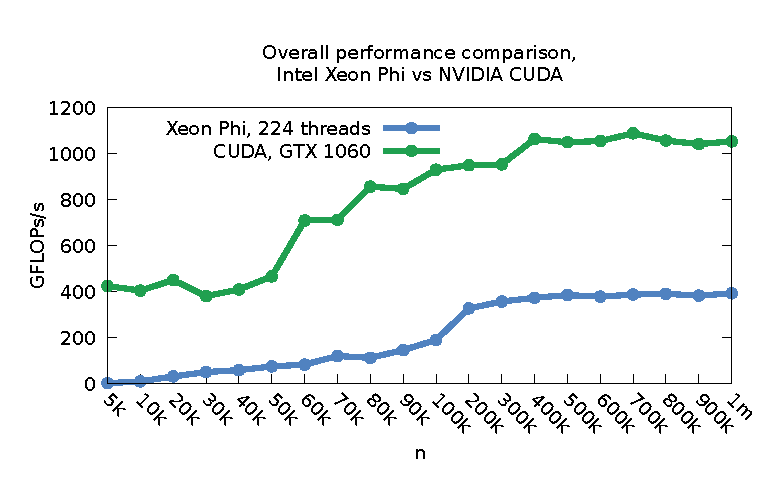
\includegraphics[width=.5\textwidth]{gnuplot/cuda.eps}
				\caption{\label{cuda}Floating-point performance comparison of Xeon Phi and GTX 1060}
			\end{figure} 
			
			Even though the GTX 1060 I ran my benchmarks on is nowhere near being the top of the line GPU, the resulting running times and corresponding computational power were still very good. For larger datasets (hundreds of thousands of bodies), I sometimes saw the floating-point performance exceed one teraflop - the highest performance I recorded was $1089$ GFLOPs/s when measuring the running time on 700 thousand bodies. Compared to the Xeon Phi benchmarking data, which gave me the best results up to that point, I was pleasantly surprised to see another 3-fold speedup. I plotted a comparison of the two devices' floating-point performance in figure \ref{cuda}.	
		
		\begin{figure}[ht]			
			\centering
			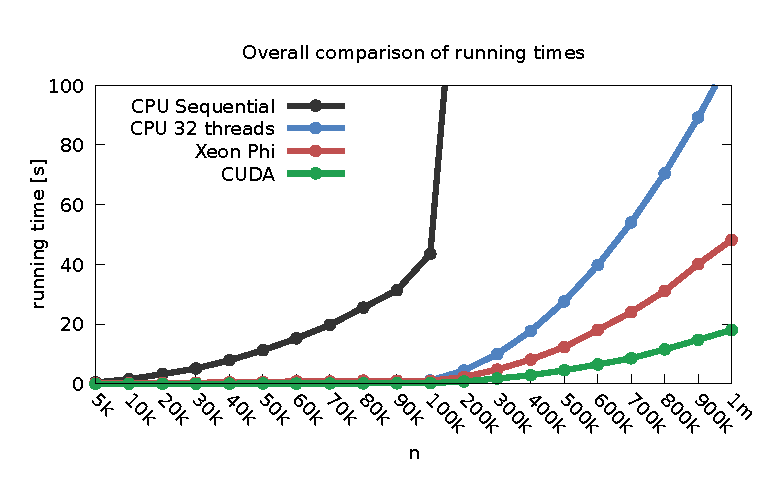
\includegraphics[width=.5\textwidth]{gnuplot/big_comparison.eps}
			\caption{\label{comparo}Running times of all implementations}
		\end{figure} 
		
		The last chart which you can see in figure \ref{comparo} denotes the final comparison of the running times of all of the N-Body simulation implementations created during this course project. 
		
		You can clearly see that approaching this problem in a naive and sequential manner is quite inefficient. This fact becomes more apparent as the number of bodies increases. A parallel approach to this problem is a good start, however the running times per iteration rise to tedious levels quite quickly as well. CUDA, on the other hand, really proved itself to be the way to go for algorithms that are embarrassingly parallel, such as this one.
		
	\section{Conclusion}
	
		In this course project for the CIS 750 - Advanced Computer Architecture Experiments course at Kansas State University, I tasked myself with implementing multiple versions of a brute-force or all-pairs algorithm that solves the N-Body simulation problem.
		
		In section \ref{algs}, I first briefly explained some specifics of what the N-Body simulation problem is. I then introduced two algorithms that are commonly used to run a simulation of this nature, listing the pros and cons for each of them. After that, I took a closer look at the brute-force (all-pairs) algorithm and explained its inner workings more thoroughly.
		
		I implemented a naive and an optimized implementation of this algorithm at first, in both sequential and parallel versions. The parallel versions were created using the OpenMP parallel programming interface. 
		
		I then continued to create an implementation that could be run on the Intel Xeon Phi coprocessor (section \ref{phisection}), and another implementation that could be run on NVIDIA's graphics processing units using CUDA technology (\ref{cudasection}). 
		
		I performed all of these implementations in either C++ or CUDA-C (CUDA implementation only). In section \ref{orangepi}, I explained an issue I had with one of my proposed tasks and why I decided to skip a part of the project altogether. 
		
		For each of these implementations, I created test scripts and used those to benchmark the application on a vast variety of dataset sizes and thread counts. I measured the running times and overall computing performance of each version of the application's source code.
		
		After the benchmarking was all done, I pooled all the resulting data that I gathered, analyzed it and commented on my findings. I largely confirmed my hypotheses that sacrificing code readability by using a Structure of Arrays kind of memory design would bring noticeable performance improvements, and that, as I showed in section \ref{phisection}, using a Xeon Phi coprocessor would yield solid speedups, despite the exact model I used in my project being quite old and relatively slow.
		
		I also found that using CUDA technology for this kind of simulation is indeed a very good idea and that its performance is very respectable. I measured a significant speedup of the simulation when running my CUDA application on a GeForce GTX 1060 GPU.\ref{cudasection}

		\subsection*{Future work directions}	
			
			I wish I could have tried to benchmark an ARM-architecture based device as well, but time management and an unexpected hardware failure forced me to not perform any tests on such a device.
			
			In the future, I think it would be beneficial to repeat the project using the Barnes-Hut algorithm (that I briefly described in section \ref{barnes}) and re-run all the benchmarks, just to see how much more efficient it really is, even if it's not as embarrassingly parallel as the brute-force algorithm.
			
	
	\bibliographystyle{ieeetr}
	\bibliography{mybibliographyfile}
	
\end{document}


